% partes/parte3/cap09.tex
\chapter{Tipos de comportamiento de compra y modelos de estudio del consumidor digital}
\label{cap:09}

\begin{cajaFicha}
\begin{description}
  \item[Unidad temática] III — Modelos de comportamiento del consumidor digital.
  \item[Temas del programa] 3.1 Tipos de comportamiento del consumidor: 3.1.1 Complejo; 3.1.2 Reductor de disonancia; 3.1.3 Habitual; 3.1.4 Variado. 3.2 Modelos de estudio del comportamiento del consumidor digital: 3.2.1 Económico de Marshall; 3.2.2 Estímulo-respuesta de Pavlov; 3.2.3 Sociológico de Veblen; 3.2.4 Psicoanalítico de Freud; 3.2.5 Acción razonada de Fishbein y Ajzen; 3.2.6 Funcional de O'Shaughnessy; 3.2.7 Motivacional (pirámide de necesidades de Maslow); 3.2.8 Integrador entrada-proceso-salida de Howard y Sheth; 3.2.9 Antropológico-etnográfico de consumo digital.
  \item[Horas] Teoría 6.0 · Práctica 12.0 · Aprendizaje autónomo 5.0 (suma de los temas 3.1 y 3.2 del programa; el capítulo cubre dos semanas de clase).
  \item[Competencia de la unidad] Distingue los modelos de estudio del comportamiento del consumidor digital con base en sus tipos y el análisis de los modelos de decisión de compra.
  \item[Resultados de aprendizaje observables] Al concluir el capítulo, el estudiante:
  \begin{enumerate}
    \item clasifica un episodio de compra en uno de los cuatro tipos (complejo, reductor de disonancia, habitual o variado) a partir del involucramiento y de las diferencias percibidas entre marcas, y explica por qué el tipo pertenece al episodio y no al producto;
    \item reconoce la firma de datos de cada tipo en una analítica digital y propone la táctica de mercadotecnia que le corresponde;
    \item explica, para cada uno de los nueve modelos, su supuesto central, su variable clave, un ejemplo digital y su límite, y distingue lo que el autor dijo de lo que los manuales le atribuyen;
    \item calcula la actitud multiatributo, la norma subjetiva y la intención de compra de tres marcas y localiza el peso social en que cambia la elección;
    \item elige, con argumentos, qué modelo (o combinación) sirve para responder una pregunta concreta de mercadotecnia digital.
  \end{enumerate}
  \item[Prerrequisitos] Cap.~1--8, en particular el proceso de decisión (Cap.~6) y las figuras participantes (Cap.~8).
\end{description}
\end{cajaFicha}

\section{Caso de apertura}

\begin{casoFicticio}
Camila, estudiante de tercer semestre, hace cuatro compras en una misma semana.

\textbf{Lunes.} Necesita una laptop para el semestre. Pasa seis noches viendo
reseñas en video, abre doce pestañas con comparadores, pregunta a su primo que
sabe de computadoras y llega a una hoja de cálculo con cuatro candidatas.
Compra la tercera. Tardó nueve días.

\textbf{Miércoles.} Pide un colchón matrimonial en una tienda en línea. Todas las
marcas le parecen \enquote{más o menos lo mismo}, pero el gasto es grande. Elige
la que tiene entrega gratis y financiamiento. Esa noche escribe en el buscador:
\enquote{colchón [marca] opiniones}. Quiere confirmar que no se equivocó.

\textbf{Viernes.} Se acaba el detergente. Abre la tienda, toca
\enquote{volver a pedir} y paga. Tardó cuarenta segundos y no miró la
marca, porque nunca la mira.

\textbf{Sábado.} Compra papas fritas. Hoy las prueba de un sabor que no
conocía, porque salió una edición limitada. No estaba insatisfecha con las de
siempre: quería algo distinto.
\end{casoFicticio}

La misma persona, con el mismo presupuesto, hizo cuatro cosas distintas. Una
analítica que la describa como \enquote{compradora en línea con ticket
promedio de tanto} borra todo lo que importa. Este capítulo da dos
herramientas para no borrarlo. La primera es una tipología: cuatro formas de
comprar, que se distinguen por cuánto se involucra la persona y cuánto
difieren las marcas a sus ojos. La segunda es un conjunto de nueve
\emph{modelos}, nueve explicaciones de por qué las personas compran, cada una
nacida en una disciplina distinta y cada una con algo que decir sobre la semana
de Camila.

Los dos bloques responden preguntas diferentes. La tipología describe
\emph{cómo} se compra (con mucha o poca deliberación). Los modelos intentan
explicar \emph{por qué} (utilidad, hábito, estatus, deseo, actitud, necesidad).
Se estudian juntos porque la tipología sirve para decidir \emph{qué modelo
conviene} aplicar a cada episodio, como se verá en la sección final del
desarrollo.

\section{Desarrollo teórico}

\subsection{Tipos de comportamiento del consumidor}

\subsubsection{Dos ejes: involucramiento y diferencias percibidas}

La tipología más usada en los textos de mercadotecnia se atribuye a Henry
Assael \parencite{assael1987}, y los manuales la reproducen como una matriz de
dos por dos. Un eje es el \emph{involucramiento} del consumidor con la compra,
alto o bajo. El otro es el grado de \emph{diferencia percibida} entre las marcas,
grande o pequeño (figura~\ref{fig:cap09-matriz}).

\begin{cajaDefinicion}
\textbf{Involucramiento.} Importancia que una persona le da a una compra
concreta, medida por cuánto esfuerzo está dispuesta a invertir en decidir. Sube
con el \emph{riesgo percibido} (financiero, social, de desempeño), con la
frecuencia baja de la compra, con su relación con la identidad de la persona y
con el costo de equivocarse.

\textbf{Diferencias percibidas entre marcas.} Cuánto distingue la persona unas
opciones de otras \emph{desde su propia mirada}, no desde la ficha técnica. Dos
colchones con construcción distinta pueden ser \enquote{lo mismo} para quien no
sabe qué comparar.
\end{cajaDefinicion}

\begin{figure}[!htb]
  \centering
  \resizebox{0.9\textwidth}{!}{% figuras/tikz/cap09-matriz-assael.tex
% Matriz 2x2 de los cuatro tipos de comportamiento de compra (Assael, 1987).
\begin{tikzpicture}[
    celda/.style={rectangle, draw=guindaIPN, thick, minimum width=5.6cm, minimum height=3.1cm,
                  align=center, font=\scriptsize, text width=5.2cm},
    eje/.style={font=\scriptsize\bfseries, text=guindaIPNOsc}
  ]
  \node[celda, fill=guindaIPNClara]    at (0,3.3)   {\textbf{\normalsize Complejo}\\[2pt] Busca, compara y aprende\\ antes de elegir.\\ \textit{Ej.: laptop, curso, seguro}};
  \node[celda, fill=bronceIPNClaro]    at (5.8,3.3) {\textbf{\normalsize Reductor de disonancia}\\[2pt] Elige rápido, duda después\\ y busca reafirmación.\\ \textit{Ej.: colchón, sofá, crédito}};
  \node[celda, fill=terracotaIPNClara] at (0,0)     {\textbf{\normalsize Variado}\\[2pt] Cambia de marca por probar,\\ no por insatisfacción.\\ \textit{Ej.: botana, bebida, serie}};
  \node[celda, fill=grisIPN!8]         at (5.8,0)   {\textbf{\normalsize Habitual}\\[2pt] Compra por rutina, casi sin\\ buscar ni evaluar.\\ \textit{Ej.: detergente, recarga}};
  \node[eje] at (0,5.3)   {Diferencias grandes entre marcas};
  \node[eje] at (5.8,5.3) {Diferencias pequeñas entre marcas};
  \node[eje, rotate=90] at (-3.2,3.3) {Involucramiento alto};
  \node[eje, rotate=90] at (-3.2,0)   {Involucramiento bajo};
\end{tikzpicture}
}
  \caption{Matriz de los cuatro tipos de comportamiento de compra. Fuente:
  elaboración propia con base en la tipología de \textcite{assael1987}.}
  \label{fig:cap09-matriz}
\end{figure}

Tres aclaraciones evitan los errores más comunes al usar la matriz.

\begin{enumerate}
  \item \textbf{El tipo no es una propiedad del producto, sino del episodio.} El
  detergente es \enquote{habitual} para Camila y puede ser \enquote{complejo} para
  una persona con piel alérgica que investiga ingredientes. La primera laptop
  fue una compra compleja; la segunda, de la misma marca tres años después, será
  habitual. Por eso la tabla de ejemplos de este capítulo habla de
  \emph{episodios}.
  \item \textbf{Es una tipología, no una ley.} Dos ejes y dos niveles por eje
  producen cuatro casillas, pero las personas se reparten en un continuo. Los
  umbrales entre \enquote{alto} y \enquote{bajo} son una convención del analista.
  El laboratorio del capítulo muestra cuánto cambian los porcentajes cuando se
  mueve el umbral.
  \item \textbf{Hay enfoques que prefieren el continuo.} \textcite{solomon2017}
  trata la complejidad de la decisión como un continuo que va de la decisión
  habitual a la extensa, con la decisión limitada en medio, y no pone en el centro
  la matriz de cuatro casillas. No es una contradicción: es otra forma de cortar
  el mismo fenómeno. \datoPendiente{contrastar este párrafo con la 11.ª edición
  física de Solomon (2017); pendiente \#15}
\end{enumerate}

\subsubsection{Complejo}
\progtag{3.1.1}
\label{sec:cap09-complejo}

Es la combinación de alto involucramiento y diferencias grandes. La persona
siente que hay mucho en juego y que elegir bien importa, porque las opciones
\emph{sí} son distintas. El proceso se parece al de cinco etapas del Cap.~6 en
su versión completa: primero forma \emph{creencias} sobre los atributos, luego
\emph{actitudes} hacia las marcas y al final elige \parencite{assael1987}.

\begin{cajaEjemplo}[title={Ejemplo digital: la laptop de Camila}]
\textbf{Qué se ve en los datos.} Doce sesiones en nueve días, de tres
dispositivos distintos; visitas a páginas de comparación, tablas de
especificaciones y reseñas en video; búsquedas de marca más \enquote{vs}; una
hoja de cálculo propia (que ninguna analítica ve); y finalmente una compra en
la tercera visita al mismo producto.

\textbf{Qué quiere la persona.} Información comparable y confiable: fichas claras,
reseñas verificadas, la posibilidad de comparar dos modelos lado a lado.

\textbf{Qué conviene hacer.} Contenido educativo (guías de compra, comparadores
honestos), atención humana en el momento de duda (chat), reseñas visibles con
sus límites y un proceso de devolución sencillo que reduzca el riesgo percibido.
\end{cajaEjemplo}

\textbf{Otros ejemplos.} Un seguro de gastos médicos, un posgrado en línea, un
sistema de punto de venta para un negocio, un teléfono que costará dos
quincenas de sueldo. En todos, el costo de equivocarse es alto y las alternativas
cambian en algo que importa (cobertura, plan de estudios, funciones, cámara).

\textbf{Error típico de la marca.} Tratar a esta persona con un anuncio
emocional de cinco segundos. Ella está \emph{buscando razones}, y un anuncio sin
información no se las da.

\subsubsection{Reductor de disonancia}
\progtag{3.1.2}
\label{sec:cap09-disonancia}

Alto involucramiento y diferencias pequeñas. La compra es importante, pero las
marcas parecen similares. La persona decide con relativa rapidez, guiada por
el precio o por la comodidad, y \emph{después} puede sentir duda: la
\emph{disonancia} posterior a la compra, la incomodidad de haber elegido entre
opciones que no se distinguían \parencite{assael1987}. Para reducirla busca
información que confirme la decisión y desatiende la que la contradice.

\begin{cajaEjemplo}[title={Ejemplo digital: el colchón de Camila}]
\textbf{Qué se ve en los datos.} Una sesión corta y decidida (precio y
financiamiento pesan más que las fichas); compra el miércoles por la tarde;
\emph{esa misma noche} regresa al sitio, busca \enquote{opiniones} de la marca que
acaba de comprar y abre el correo de confirmación varias veces. En las semanas
siguientes, las devoluciones dentro del plazo de arrepentimiento son el
indicador de disonancia no resuelta.

\textbf{Qué quiere la persona.} Confirmación y tranquilidad: que otras personas
hayan elegido lo mismo y estén contentas, garantías, atención si algo sale
mal.

\textbf{Qué conviene hacer.} Correos posteriores a la compra con
validación (qué esperar, cómo cuidar el producto), reseñas de personas
compradoras, garantía visible, un contacto humano ante cualquier duda. La
mercadotecnia aquí no termina en el pago: \emph{empieza} ahí.
\end{cajaEjemplo}

\textbf{Otros ejemplos.} Un sofá, un seguro de auto con precios casi iguales, un
crédito personal, la matrícula de una universidad cuando las opciones parecen
equivalentes.

\begin{cajaAtencion}
Que el mensaje de después de la compra \enquote{reduzca la disonancia} es
distinto de que \emph{manipule}. Confirmar con información veraz que la
persona eligió bien (garantía, soporte, cuidado del producto) ayuda. Ocultar
reseñas negativas o inflar las positivas para que no dude, no.
\end{cajaAtencion}

\subsubsection{Habitual}
\progtag{3.1.3}
\label{sec:cap09-habitual}

Bajo involucramiento y diferencias pequeñas. La persona no busca información,
no compara y no forma una actitud profunda; compra lo que conoce porque es lo
que está a mano. Lo que parece \enquote{lealtad} puede ser simplemente
\emph{inercia}: nadie la eligió, nadie la defendería si cambiara el estante
\parencite{assael1987}.

\begin{cajaEjemplo}[title={Ejemplo digital: el detergente de Camila}]
\textbf{Qué se ve en los datos.} Cuarenta segundos entre abrir la tienda y pagar;
una sola página vista; entrada directa o desde el botón de \enquote{volver a
pedir}; cero búsquedas de marca; una recompra cada cinco o seis semanas con
regularidad casi mecánica.

\textbf{Qué quiere la persona.} Que no cambie nada: el mismo producto, en el mismo
lugar, con el menor esfuerzo.

\textbf{Qué conviene hacer.} Reducir fricción: recompra de un toque, suscripción
con aviso, \enquote{el predeterminado}, disponibilidad. Atención: lo que la
analítica llama \enquote{cliente fiel} aquí puede desaparecer si un competidor
simplemente aparece primero en la lista del asistente de compra.
\end{cajaEjemplo}

\textbf{Otros ejemplos.} La recarga de saldo, el papel higiénico, la leche, la
aplicación de transporte que siempre se abre primero, la suscripción que se
renueva sola.

\begin{cajaAtencion}
La compra habitual es el terreno donde más se prestan los \textit{patrones
oscuros} del Cap.~6: renovaciones automáticas difíciles de cancelar, casillas
premarcadas, cobros recurrentes que la persona ya no recuerda. Como no hay
deliberación, no hay oportunidad de que la persona se detenga a evaluar. El
recuadro de ética del capítulo regresa a este punto.
\end{cajaAtencion}

\subsubsection{Variado}
\progtag{3.1.4}
\label{sec:cap09-variado}

Bajo involucramiento y diferencias grandes. A la persona no le importa mucho
el producto, pero las marcas son claramente distintas. Cambia de marca con
frecuencia, y no porque esté insatisfecha, sino \emph{por variedad}: por
probar, por curiosidad, por aburrimiento \parencite{assael1987}. Es el tipo
más difícil de \enquote{fidelizar} y el más fácil de interrumpir con una novedad.

\begin{cajaEjemplo}[title={Ejemplo digital: las papas de Camila}]
\textbf{Qué se ve en los datos.} Compras frecuentes de ticket bajo, con una marca
distinta cada vez; búsqueda de \enquote{nuevo sabor} o clic en una promoción de
edición limitada; poca o ninguna lectura de reseñas; una alta tasa de cambio
de marca \emph{sin} queja previa.

\textbf{Qué quiere la persona.} Algo nuevo, sin complicaciones.

\textbf{Qué conviene hacer.} Para quien lidera la categoría, ocupar el
estante digital con variedad propia (sabores, ediciones limitadas, paquetes
mixtos) y no con descuentos. Para la marca retadora, muestras, tamaños de
prueba y presencia de novedad en las primeras posiciones.
\end{cajaEjemplo}

\textbf{Otros ejemplos.} Un refresco o una bebida energética, la música que se
descubre en una plataforma, una serie que se elige por la portada, una receta
nueva cada semana, un videojuego móvil gratuito.

\subsubsection{Los cuatro tipos en la analítica}

El cuadro~\ref{tab:cap09-tipos} reúne lo anterior para que el analista pueda
reconocer cada tipo a partir de sus datos. Son \emph{indicios}, no pruebas: lo
que se observa es el comportamiento, y el involucramiento y las diferencias
percibidas son estados mentales que se infieren.

\begin{table}[!htb]
\centering
\footnotesize
\begin{tabular}{@{}>{\raggedright}p{2.0cm}>{\raggedright}p{3.0cm}>{\raggedright}p{3.4cm}>{\raggedright\arraybackslash}p{3.6cm}@{}}
\toprule
Tipo & Firma en los datos & Qué busca la persona & Táctica principal \\
\midrule
Complejo & Muchas sesiones y dispositivos; comparadores y reseñas; ciclo largo (días o semanas) & Información comparable y confiable & Contenido educativo, comparadores, chat, devolución sencilla \\
Reductor de disonancia & Sesión corta y decidida; regreso tras la compra; búsqueda de opiniones posterior; devoluciones & Confirmación y tranquilidad & Mensajes posteriores a la compra, garantía, soporte \\
Habitual & Una página, entrada directa, recompra regular, cero búsqueda de marca & Que no cambie nada & Recompra de un toque, suscripción, disponibilidad \\
Variado & Cambio de marca sin queja previa; clic en novedades; ticket bajo & Probar algo distinto & Variedad, ediciones limitadas, muestras \\
\bottomrule
\end{tabular}
\caption{Firma en los datos y táctica de cada tipo de comportamiento de
compra. Fuente: elaboración propia con base en \textcite{assael1987}; las
firmas son indicios para el análisis, no resultados de un estudio.}
\label{tab:cap09-tipos}
\end{table}

\subsubsection{Cuando el entorno digital cambia el tipo}

La tipología tiene una consecuencia incómoda para el comercio electrónico: la
interfaz puede \emph{mover} un episodio de un cuadrante a otro.

\begin{itemize}
  \item Un comparador que ordena las opciones por precio y las vuelve
  comparables baja la \emph{diferencia percibida}: empuja las compras
  complejas hacia la disonancia (se elige por precio, y la duda aparece después).
  \item El pago de un toque y la recompra automática bajan el
  \emph{involucramiento}: empujan hacia lo habitual compras que antes se pensaban.
  \item Un asistente de compra que recomienda una sola opción hace lo mismo y
  concentra la elección en quien programó la recomendación (ver el recuadro
  de Frontera al final del desarrollo).
  \item Un lanzamiento constante de novedades sube la \emph{diferencia percibida}
  en categorías de bajo involucramiento: lo habitual se vuelve variado.
\end{itemize}

Es decir, el tipo de comportamiento no es solo algo que la persona \enquote{trae};
también es algo que el diseño de la plataforma \emph{produce}. Esa idea
reaparece en el Cap.~6 (arquitectura de la decisión) y en la ética de este
capítulo.

\begin{cajaFrontera}
\textbf{Vigente a noviembre de 2026: ¿quién tiene el involucramiento cuando
compra un agente?} Cada vez más asistentes basados en modelos de lenguaje
buscan, comparan y, en algunos casos, ejecutan compras en nombre de la persona
(Cap.~4). Si la persona delega una compra de bajo involucramiento, el
comportamiento que se observa en los datos es el del \emph{agente}, no el de la
persona, y la tipología pierde su indicio principal. Las cifras de adopción de
estos asistentes provienen de blogs de la industria y no se reportan en este
libro como dato verificado (pendiente \#13). La pregunta metodológica sí es
estable: antes de clasificar a alguien en un cuadrante, ¿se sabe quién (o qué)
hizo la compra?
\end{cajaFrontera}

\subsection{Modelos de estudio del comportamiento del consumidor digital}

\subsubsection{Qué es un modelo y por qué hay nueve}

Un modelo es una representación simplificada que destaca \emph{algunas} causas
de un fenómeno y deja las demás fuera. Ninguno es \enquote{el correcto}: cada
uno ilumina una parte de la decisión y oscurece otra. El programa propone nueve
(figura~\ref{fig:cap09-linea}), y conviene saber desde el inicio tres cosas
sobre ellos.

\begin{figure}[!htb]
  \centering
  \resizebox{\textwidth}{!}{% figuras/tikz/cap09-linea-modelos.tex
% Los nueve modelos del programa en su fecha de origen (obra de referencia) y disciplina base.
\begin{tikzpicture}[
    mod/.style={rectangle, rounded corners, draw=guindaIPN, thick, fill=guindaIPNClara, align=center,
                font=\scriptsize, minimum width=2.5cm, minimum height=0.95cm},
    met/.style={rectangle, rounded corners, draw=bronceIPN, thick, fill=bronceIPNClaro, align=center,
                font=\scriptsize, minimum width=2.5cm, minimum height=0.95cm},
    ano/.style={font=\scriptsize\bfseries, text=guindaIPNOsc}
  ]
  \draw[-{Stealth[length=2.5mm]}, thick, draw=doradoIPN] (-0.3,0) -- (15.2,0);
  % x escalado: 1890 -> 0, 2002 -> 14.5 (aprox. lineal)
  \foreach \x/\y/\txt/\est in {
      0.0/1.3/{Marshall\\ económico}/mod,
      1.2/-1.4/{Veblen\\ sociológico}/mod,
      3.6/1.3/{Pavlov\\ estímulo-respuesta}/mod,
      5.0/-1.4/{Maslow\\ motivacional}/mod,
      6.2/1.3/{Dichter (Freud)\\ psicoanalítico}/mod,
      8.4/-1.4/{Howard-Sheth\\ integrador}/mod,
      9.5/1.3/{Fishbein-Ajzen\\ acción razonada}/mod,
      11.6/-1.4/{O'Shaughnessy\\ funcional}/mod,
      13.8/1.3/{Kozinets\\ netnografía (método)}/met}
    { \node[\est] (n) at (\x,\y) {\txt}; \draw[thick, draw=grisIPN] (\x,0) -- (n); \fill[guindaIPN] (\x,0) circle (2pt); }
  \node[ano] at (0.0,-0.35)  {1890};
  \node[ano] at (1.2,0.35)   {1899};
  \node[ano] at (3.6,-0.35)  {1927};
  \node[ano] at (5.0,0.35)   {1943};
  \node[ano] at (6.2,-0.35)  {\textasciitilde 1950};
  \node[ano] at (8.4,0.35)   {1969};
  \node[ano] at (9.5,-0.35)  {1975};
  \node[ano] at (11.6,0.35)  {1987};
  \node[ano] at (13.8,-0.35) {2002};
\end{tikzpicture}
}
  \caption{Los nueve modelos en la fecha de su obra de referencia. El año de
  Pavlov es el de la edición inglesa académica de sus lecciones (1927), no el de
  sus primeros experimentos; el de Dichter es aproximado (años cincuenta del
  siglo XX). Fuente: elaboración propia con base en \textcite{marshall1890,
  veblen1899,pavlov1927,maslow1943,dichter1960,howardsheth1969,fishbein1975,
  oshaughnessy1987,kozinets2002}.}
  \label{fig:cap09-linea}
\end{figure}

\begin{enumerate}
  \item \textbf{La mayoría no nació como teoría del consumidor.} Marshall
  escribió economía; Pavlov, fisiología; Veblen, sociología de las
  instituciones; Freud, psicología clínica. La lectura \enquote{de
  mercadotecnia} de esos autores es una reconstrucción posterior hecha por
  manuales. Es útil, pero hay que presentarla como lo que es: ninguno de ellos
  escribió sobre mercados digitales, y ninguno escribió pensando en un
  \enquote{consumidor} en el sentido del siglo XX.
  \item \textbf{No son del mismo tipo.} Los hay que explican por qué se compra
  (Marshall, Veblen, Maslow), los que describen cómo se aprende (Pavlov), los
  que predicen una conducta (Fishbein y Ajzen), los que integran variables
  (Howard y Sheth) y uno que es un \emph{método} de investigación, no una
  teoría (la netnografía). El libro lo señala cuando llega.
  \item \textbf{Se complementan.} Cada modelo responde bien una pregunta
  y mal otras. La sección final del desarrollo ofrece una guía para elegir.
\end{enumerate}

Para que las diferencias se vean, el capítulo recorre los nueve con \emph{el mismo
caso}. Camila quiere comprar unos audífonos inalámbricos. Cada modelo mira ese
mismo hecho con una lente distinta.

\subsubsection{Modelo económico de Marshall}
\progtag{3.2.1}
\label{sec:cap09-marshall}

\textbf{Idea.} La persona actúa para obtener la mayor satisfacción (utilidad)
posible con un presupuesto limitado. Cada unidad adicional de un bien le da
menos satisfacción que la anterior (\emph{utilidad marginal decreciente}), y
reparte su gasto hasta que el último peso rinde lo mismo en todos los usos
\parencite{marshall1890}. Marshall introduce además el \emph{excedente del
consumidor}: la diferencia entre lo que la persona estaría dispuesta a pagar y lo
que paga.

\begin{cajaEjemplo}[title={Ejemplo 1: utilidad marginal y la tercera taza}]
Una persona asigna a cada taza de café en una cafetería en línea una
satisfacción de 10, 6 y 2 unidades (las \enquote{útiles} son una escala
inventada). Si cada taza cuesta 5 unidades de satisfacción equivalente, compra la
primera (10 > 5) y la segunda (6 > 5), pero no la tercera (2 < 5). El
\emph{excedente} es $(10-5)+(6-5)=6$ unidades. En el comercio electrónico, un
cupón de \enquote{2 por 1} funciona porque la segunda unidad tiene todavía
utilidad marginal por encima del precio.
\end{cajaEjemplo}

\begin{cajaEjemplo}[title={Ejemplo 2: elasticidad de una suscripción}]
Una plataforma de \textit{streaming} ficticia sube su precio de 149 a 179
pesos al mes (un aumento de $(179-149)/149 \approx 20.1$\,\%) y sus suscriptores
bajan de 10\,000 a 9\,000 ($-10$\,\%). La elasticidad precio es
\[
  \varepsilon = \frac{-0.100}{+0.201} \approx -0.50.
\]
Como $|\varepsilon| < 1$, la demanda es \emph{inelástica}: el ingreso sube
(de 1\,490\,000 a 1\,611\,000 pesos al mes) aunque haya menos suscriptores. Con
$|\varepsilon|>1$ habría ocurrido lo contrario. Todos los datos son
ilustrativos.
\end{cajaEjemplo}

\textbf{Lente sobre Camila.} Compara tres pares de audífonos por precio y
batería, y elige el de mejor relación calidad-precio. Dato observable: uso de
comparadores y filtros de precio.

\textbf{Dónde falla.} El consumidor real no es el \emph{homo economicus}:
\textcite{simon1955} habló de \emph{racionalidad limitada} y
\textcite{tverskykahneman1974} documentaron heurísticas y sesgos que desvían la
decisión del óptimo (anclajes de precio, escasez artificial, \textit{nudges} de
pago, como en el Cap.~6). El modelo tampoco contiene variables sociales ni
emocionales. Su lectura para el comercio electrónico es una
\emph{extrapolación} de manuales, no una tesis de Marshall.

\subsubsection{Modelo estímulo-respuesta de Pavlov}
\progtag{3.2.2}
\label{sec:cap09-pavlov}

\textbf{Idea.} El aprendizaje por asociación: si un estímulo neutro se presenta
varias veces junto con un estímulo que ya provoca una respuesta, el neutro
termina provocando respuesta por sí mismo \parencite{pavlov1927}. Hay cuatro
piezas: estímulo incondicionado (EI), respuesta incondicionada (RI), estímulo
condicionado (EC) y respuesta condicionada (RC). Si el EC deja de acompañarse
del EI, la respuesta se apaga (\emph{extinción}).

\begin{cajaEjemplo}[title={Ejemplo: el sonido de la aplicación de ofertas}]
Una aplicación ficticia de ofertas relámpago envía una notificación con un sonido
característico (EC) \emph{siempre} que hay una oferta real (EI), que genera
emoción y atención (RI). Tras varias semanas, el sonido por sí solo (RC) produce
anticipación y apertura de la aplicación. Esa es la asociación.

\emph{Extinción}: si la aplicación empieza a mandar el sonido sin oferta
de verdad, la asociación se debilita y la gente deja de abrirla. \emph{Abuso}:
un sonido de marca que se asocia con presión de tiempo falsa (\enquote{¡solo
quedan 2!}) usa el mismo mecanismo para empujar compras. La diferencia entre
ambos usos es ética, no técnica.
\end{cajaEjemplo}

\textbf{Lente sobre Camila.} Los audífonos que ve en cada video de su creadora
favorita (música agradable, ambiente que le gusta) acumulan afecto por
repetición, antes de que ella los evalúe.

\textbf{Dónde falla.} El condicionamiento simple subestima cognición, atención y
contexto, y los resultados de los experimentos con consumidores son mixtos; el
efecto se extingue si la asociación no se refuerza. La base conceptual
del \textit{retargeting} y de la repetición de estímulos de marca es esta,
pero la evidencia de su eficacia específica en entornos digitales es más
escasa que la retórica de la industria. Además, 1927 es el año de la edición
inglesa, no del descubrimiento; la obra experimental es anterior.

\subsubsection{Modelo sociológico de Veblen}
\progtag{3.2.3}
\label{sec:cap09-veblen}

\textbf{Idea.} Consumir no solo satisface necesidades: \emph{comunica posición
social}. Veblen describe el \emph{consumo conspicuo}, el gasto visible y no
necesariamente útil cuyo propósito es mostrar estatus, y la
\emph{emulación pecuniaria}, la tendencia de cada grupo a imitar al que está
arriba \parencite{veblen1899}.

\begin{cajaEjemplo}[title={Ejemplo: la edición limitada que se muestra}]
Unos tenis de edición limitada cuestan 4\,800 pesos; los modelos básicos de la
misma marca, 1\,900. La diferencia de funcionalidad es pequeña. Quien los compra los
publica en una historia con la etiqueta de la tienda, un \textit{unboxing} y la
ubicación de la fila. La publicación es parte del producto: sin ella, el
gasto pierde buena parte de su sentido social. Un bien así puede tener una
demanda que \emph{no} baja cuando el precio sube, porque el precio alto es parte
del mensaje.

\textbf{Qué se ve en los datos.} Compartir la compra en redes; interacciones
por \enquote{lo más caro}; búsqueda de \enquote{réplicas} entre quienes no
pueden pagar el original (emulación).
\end{cajaEjemplo}

\textbf{Lente sobre Camila.} Los audífonos de la marca que usan las
personas que ella admira son más atractivos \emph{porque} son visibles.

\textbf{Dónde falla.} La obra es un ensayo sociológico sobre la clase alta
estadounidense de finales del siglo XIX, no un estudio empírico de compra
individual. Decir que \enquote{Veblen predijo Instagram} es una lectura
retrospectiva, no algo que su texto afirme. Además, no todo el consumo de
estatus es visible: existe el consumo de estatus \enquote{silencioso}.

\subsubsection{Modelo psicoanalítico de Freud (y su mediación por Dichter)}
\progtag{3.2.4}
\label{sec:cap09-freud}

\begin{cajaAtencion}
\textbf{Corrección conceptual.} El programa dice \enquote{psicoanalítico de
Freud}, pero Sigmund Freud \emph{no escribió sobre el comportamiento del
consumidor}. El modelo que llega a la mercadotecnia pasa por Ernest Dichter,
quien trasladó ideas psicoanalíticas (motivos inconscientes, simbolismo del
producto) a la investigación de mercado a través de la \emph{investigación
motivacional}, popularizada sobre todo en los años cincuenta en Estados Unidos
\parencite{dichter1960,schwarzkopf2015dichter}. La cadena es: psicoanálisis
clínico $\rightarrow$ Dichter $\rightarrow$ investigación motivacional. Y la
historia académica es cautelosa con la afirmación de que Dichter fue su único
origen.
\end{cajaAtencion}

\textbf{Idea.} Parte de las compras responde a motivos que la persona no
reconoce o no puede decir en una encuesta directa. Los productos funcionan como
símbolos con significado psicológico.

\begin{cajaEjemplo}[title={Ejemplo: la aplicación de pagos}]
En una encuesta, jóvenes dicen que usan una aplicación de pagos porque es
\enquote{rápida}. En una entrevista en profundidad con una técnica proyectiva
(\enquote{complete la frase: la persona que gasta sin controlar es\ldots})
aparece otra cosa: el miedo a perder el control del dinero. La aplicación que
muestra un resumen semanal del gasto responde a ese motivo, que ningún
cuestionario cerrado habría recogido.
\end{cajaEjemplo}

\textbf{Lente sobre Camila.} Los audífonos de cancelación de ruido pueden
significar para ella \enquote{mi espacio}, un refugio frente a un entorno
saturado, algo que ella no diría al llenar un formulario.

\textbf{Dónde falla.} El método es difícil de replicar y de validar
estadísticamente, y su vínculo con el psicoanálisis freudiano se ha criticado
como oportunismo comercial más que como rigor científico. Su legado actual
son las técnicas cualitativas: entrevistas en profundidad de UX, el
\textit{insight} de marca. Esa continuidad metodológica es razonable, pero no es
una cita de Dichter sobre medios digitales.

\subsubsection{Modelo de acción razonada de Fishbein y Ajzen}
\progtag{3.2.5}
\label{sec:cap09-fishbein}

\textbf{Idea.} La mejor predicción de una conducta es la \emph{intención}, que
depende de dos factores: la \emph{actitud} hacia hacerla y la \emph{norma
subjetiva}, la presión social que la persona percibe \parencite{fishbein1975}.
Ajzen agregó después el \emph{control conductual percibido} (la facilidad o
dificultad que la persona ve en la conducta) y llamó al modelo ampliado
\emph{teoría de la conducta planeada} \parencite{ajzen1991}. Los estudios
comparativos encuentran que la versión ampliada predice mejor cuando la
persona no tiene control total sobre la conducta \parencite{madden1992}.

\begin{cajaDefinicion}
\textbf{Actitud multiatributo.} Suma, sobre los atributos $i$ de una marca, del
producto entre la \emph{creencia} $b_i$ (qué tan probable es que la marca tenga
el atributo) y la \emph{evaluación} $e_i$ (qué tan bueno es ese atributo para la
persona):
\[
  A = \sum_i b_i\, e_i .
\]
\textbf{Norma subjetiva.} Suma, sobre los referentes $k$, del producto entre la
\emph{creencia normativa} $nb_k$ (cuánto aprueba el referente la conducta) y la
\emph{motivación para complacerlo} $mc_k$:
\[
  SN = \sum_k nb_k\, mc_k .
\]
\textbf{Intención.} $BI = w_A\,A + w_N\,SN$, con pesos $w_A, w_N$ que se
estiman con datos. En el laboratorio, $A$ y $SN$ se reescalan a $[-1,1]$ para
poder sumarlos.
\end{cajaDefinicion}

\begin{cajaEjemplo}[title={Ejemplo con números: los audífonos de Camila}]
Camila valora cuatro atributos: precio accesible ($e=+3$), batería ($+2$), sonido
($+2$) y reseñas ($+1$). Cree que las tres marcas ficticias tienen cada
atributo con las probabilidades $b$ (de 0 a 10) de esta tabla:

\begin{center}
\footnotesize
\begin{tabular}{@{}lcccc|c@{}}
\toprule
 & Precio & Batería & Sonido & Reseñas & $A=\sum b\,e$ \\
\midrule
$e$ & $+3$ & $+2$ & $+2$ & $+1$ & \\
Marca A (económica) & 9 & 5 & 3 & 5 & $27+10+6+5=48$ \\
Marca B (equilibrada) & 6 & 7 & 6 & 7 & $18+14+12+7=51$ \\
Marca C (premium) & 2 & 8 & 9 & 8 & $6+16+18+8=48$ \\
\bottomrule
\end{tabular}
\end{center}

Solo por actitud, gana la B (51 frente a 48). Ahora, tres personas importan:
sus amistades, la creadora de contenido que sigue y su familia, con motivación
para complacerlas de 6, 8 y 4. La creadora recomienda con fuerza la C y a su
familia le gusta la A. La norma subjetiva sale en 20 para A, 18 para B y 22 para
C. Con pesos $w_A=0.6$ y $w_N=0.4$ la intención de la C pasa a ser la más alta,
por un margen mínimo (0.523 frente a 0.516 de la B). Es la lección: una elección
que parece clara por actitud puede cambiar por presión social, y los márgenes
pueden ser muy pequeños. El laboratorio de este capítulo reproduce estas cifras.
\end{cajaEjemplo}

\textbf{Lente sobre Camila.} Pregunta qué piensan sus amistades (norma),
evalúa atributos (actitud) y se sabe capaz de pagar (control percibido).

\textbf{Dónde falla.} Supone procesamiento deliberado: subestima hábitos,
emociones y procesos automáticos, y la \emph{brecha entre intención y
conducta} es una limitación bien conocida: la intención declarada en una
encuesta no siempre llega al carrito, y el carrito no siempre llega al pago.
Es, con Howard y Sheth, el modelo del capítulo con más trazabilidad hacia la
literatura digital: el modelo de aceptación de tecnología (TAM) se deriva de la acción razonada.

\subsubsection{Modelo funcional de O'Shaughnessy}
\progtag{3.2.6}
\label{sec:cap09-oshaughnessy}

\textbf{Idea.} \textcite{oshaughnessy1987} critica los modelos
\enquote{mecanicistas} y la sobredependencia de la elección racional. Sostiene
que la razón que la persona da es muchas veces una \emph{justificación posterior}
de una decisión tomada por vía emocional, que los \emph{deseos} y las
\emph{necesidades} son cosas distintas (se puede desear lo que no se necesita
y necesitar lo que no se desea), y que a veces la persona no sabe qué desea
hasta que un estímulo se lo recuerda.

\begin{cajaEjemplo}[title={Ejemplo: el reloj inteligente}]
Una persona dice que compró un reloj inteligente \enquote{para monitorear mi
salud} (razón funcional). Pero en la entrevista cuenta que su grupo de
corredores lo usa y que se sentía fuera de la conversación (razón de
pertenencia). La razón declarada es una justificación posterior.

\textbf{Qué se ve en los datos.} Reseñas que hablan de \enquote{comunidad} y de
\enquote{motivación} más que de funciones; devoluciones de quienes lo compraron
\enquote{por la función} y no la usan; el uso real del dispositivo contra lo que la persona
dijo al comprarlo.
\end{cajaEjemplo}

\begin{center}
\footnotesize
\begin{tabular}{@{}lll@{}}
\toprule
 & \textbf{La necesita} & \textbf{No la necesita} \\
\midrule
\textbf{La desea} & Laptop para clases & Quinta bocina portátil \\
\textbf{No la desea} & Seguro de gastos médicos & Cuarto cargador \\
\bottomrule
\end{tabular}
\end{center}

\textbf{Lente sobre Camila.} Dirá que compra los audífonos \enquote{para la
biblioteca}. Quizá lo que busca es dejar de oír el ruido de casa.

\textbf{Dónde falla.} Es más filosófico e interpretativo que predictivo; es
difícil de contrastar empíricamente. No se localizó literatura que lo aplique de
forma nombrada a entornos digitales: su relevancia aquí es una advertencia
\emph{conceptual} (un clic o una conversión no revelan la motivación detrás), es
decir, una extrapolación pedagógica, no un hallazgo empírico.

\subsubsection{Modelo motivacional de Maslow}
\progtag{3.2.7}
\label{sec:cap09-maslow}

\begin{cajaAtencion}
\textbf{Corrección conceptual.} La \enquote{pirámide de Maslow} que aparece en
los manuales \emph{no está} en el artículo original \parencite{maslow1943}: el
texto de 1943 no contiene un diagrama. La pirámide es una simplificación
posterior, atribuida de forma habitual a un gráfico de 1960 hecho por otra
persona. Además, Maslow no planteó que los niveles se satisfagan uno por uno,
completos, antes de pasar al siguiente: una persona puede tener parcialmente
satisfechas las necesidades de varios niveles a la vez. Se presenta aquí
la teoría de 1943 y se nombra la pirámide como lo que es: una representación
popular.
\end{cajaAtencion}

\textbf{Idea.} Las necesidades humanas se organizan en cinco grupos
(fisiológicas, de seguridad, de pertenencia y amor, de estima y de
autorrealización). Las de un nivel inferior tienden a predominar mientras estén
poco satisfechas, pero la satisfacción es gradual y coexiste entre niveles
\parencite{maslow1943}.

\begin{table}[!htb]
\centering
\footnotesize
\begin{tabular}{@{}>{\raggedright}p{2.8cm}>{\raggedright}p{4.3cm}>{\raggedright\arraybackslash}p{5.0cm}@{}}
\toprule
Necesidad & Compra o uso digital & Mensaje que le corresponde \\
\midrule
Fisiológica & Pedido de comida a domicilio, farmacia en línea & Rapidez, disponibilidad \\
Seguridad & Banca móvil, seguros, copias de seguridad, pago protegido & Confianza, garantías, privacidad \\
Pertenencia & Grupos de mensajería, comunidades, regalos entre amistades & \enquote{Eres parte de\ldots} \\
Estima & Insignias, nivel en un programa de lealtad, reconocimiento de seguidores & Estatus, logro, reconocimiento \\
Autorrealización & Cursos en línea, creación de contenido, herramientas creativas & Crecimiento, propósito \\
\bottomrule
\end{tabular}
\caption{Necesidades de Maslow (1943) y ejemplos de conducta digital. Fuente:
elaboración propia con base en \textcite{maslow1943}; la correspondencia con
compras digitales es una traslación conceptual, no un hallazgo del texto
original.}
\label{tab:cap09-maslow}
\end{table}

\textbf{Lente sobre Camila.} Los audífonos pueden servirle para varias cosas
a la vez: concentrarse (logro), conversar con su grupo en una llamada
(pertenencia), sentirse en control de su entorno (seguridad).

\textbf{Dónde falla.} La base empírica original es débil (fue una teoría
basada en observación clínica), la secuencia estricta es difícil de validar
entre culturas y los manuales de mercadotecnia la distorsionan. Se usa con
provecho como \emph{heurística} para segmentar mensajes por tipo de necesidad.

\subsubsection{Modelo integrador de Howard y Sheth}
\progtag{3.2.8}
\label{sec:cap09-howard}

\textbf{Idea.} Es el primer intento serio de integrar, en un solo esquema,
las influencias cognitivas, sociales y de mercadotecnia sobre la compra
\parencite{howardsheth1969}. (El programa oficial escribe \enquote{Howarth-Sheth};
la grafía correcta del primer apellido es \emph{Howard}.) El modelo distingue
cuatro grupos de variables, como muestra la figura~\ref{fig:cap09-howard}:
\emph{entradas} (estímulos de producto, simbólicos y sociales), \emph{constructos
de proceso} (percepción y aprendizaje), \emph{salidas} (atención, comprensión de
marca, actitud, intención y compra) y \emph{variables exógenas} (importancia de la
compra, personalidad, presión de tiempo, clase social, cultura).

\begin{figure}[!htb]
  \centering
  \resizebox{0.95\textwidth}{!}{% figuras/tikz/cap09-howard-sheth.tex
% Esquema entrada-proceso-salida inspirado en Howard y Sheth (1969), simplificado.
\begin{tikzpicture}[
    ent/.style={rectangle, rounded corners, draw=bronceIPN, thick, fill=bronceIPNClaro, align=center,
                font=\scriptsize, minimum width=3.3cm, minimum height=1.0cm},
    pro/.style={rectangle, rounded corners, draw=guindaIPN, thick, fill=guindaIPNClara, align=center,
                font=\scriptsize, minimum width=3.3cm, minimum height=1.0cm},
    sal/.style={rectangle, rounded corners, draw=colorLaboratorio, thick, fill=colorLaboratorio!8, align=center,
                font=\scriptsize, minimum width=2.6cm, minimum height=0.8cm},
    exo/.style={rectangle, dashed, draw=grisIPN, align=center, font=\scriptsize, minimum width=12.5cm, minimum height=0.8cm},
    flecha/.style={-{Stealth[length=2.3mm]}, thick, draw=doradoIPN},
    tit/.style={font=\small\bfseries, text=guindaIPNOsc}
  ]
  \node[tit] at (0,4.4) {Entradas};
  \node[tit] at (5.2,4.4) {Proceso (constructos)};
  \node[tit] at (10.6,4.4) {Salidas};
  \node[ent] (e1) at (0,3.3) {Estímulos de producto\\ (precio, calidad, disponibilidad)};
  \node[ent] (e2) at (0,2.0) {Estímulos simbólicos\\ (anuncio, reseña, marca)};
  \node[ent] (e3) at (0,0.7) {Estímulos sociales\\ (familia, grupo, clase)};
  \node[pro] (p1) at (5.2,3.1) {Percepción\\ (atención, búsqueda de información)};
  \node[pro] (p2) at (5.2,1.3) {Aprendizaje\\ (motivos, criterios, confianza)};
  \node[sal] (s1) at (10.6,3.3) {Atención};
  \node[sal] (s2) at (10.6,2.45) {Comprensión de marca};
  \node[sal] (s3) at (10.6,1.6) {Actitud};
  \node[sal] (s4) at (10.6,0.75) {Intención};
  \node[sal, fill=colorLaboratorio!25] (s5) at (10.6,-0.1) {Compra};
  \draw[flecha] (e1.east) -- (p1.west); \draw[flecha] (e2.east) -- (p1.west); \draw[flecha] (e3.east) -- (p2.west);
  \draw[flecha] (e2.east) -- (p2.west);
  \draw[flecha] (p1.south) -- (p2.north);
  \draw[flecha] (p2.east) -- (s3.west); \draw[flecha] (p1.east) -- (s1.west);
  \draw[flecha] (s1) -- (s2); \draw[flecha] (s2) -- (s3); \draw[flecha] (s3) -- (s4); \draw[flecha] (s4) -- (s5);
  \draw[flecha, dashed] (s5.south) -- ++(0,-0.45) -| (5.2,-0.45) -- (p2.south |- 0,0.3) ;
  \node[font=\scriptsize\itshape, text=grisIPN] at (7.7,-0.75) {retroalimentación: la compra y su resultado vuelven a alimentar el aprendizaje};
  \node[exo] at (5.2,-1.6) {\textbf{Variables exógenas:} importancia de la compra, personalidad, presión de tiempo, clase social, cultura};
\end{tikzpicture}
}
  \caption{Esquema entrada-proceso-salida inspirado en Howard y Sheth,
  simplificado. Fuente: elaboración propia con base en
  \textcite{howardsheth1969}.}
  \label{fig:cap09-howard}
\end{figure}

\begin{cajaEjemplo}[title={Ejemplo: la consola de Valeria, vista como sistema}]
Retomamos el caso del Cap.~8. \emph{Entradas}: el precio y las
características de la consola (producto); los videos de la creadora y los
anuncios (simbólicos); la opinión de su padre y su tía (sociales).
\emph{Proceso}: Valeria presta atención a ciertos videos, compara modelos y
aprende qué criterios importan. \emph{Salidas}: reconoce la marca, forma una
actitud favorable, tiene intención y (con la tarjeta de la tía) compra.
\emph{Exógenas}: el presupuesto del hogar, la fecha de su cumpleaños.
Después de comprar, su experiencia regresa al aprendizaje y condiciona la
siguiente compra.
\end{cajaEjemplo}

\textbf{Lente sobre Camila.} Los \emph{touchpoints} son entradas, la
navegación y la comparación son proceso, la conversión es salida. De ahí que
el modelo se relacione de forma natural con el recorrido (Cap.~7), aunque Howard
y Sheth escribieron en 1969, sin comercio electrónico.

\textbf{Dónde falla.} Es complejo y sus constructos son difíciles de medir con
instrumentos válidos; su capacidad predictiva se ha cuestionado frente a modelos
más sencillos como el de acción razonada. Se cita más como marco conceptual que
como modelo aplicado.

\subsubsection{Modelo antropológico-etnográfico: la netnografía}
\progtag{3.2.9}
\label{sec:cap09-netno}

\begin{cajaAtencion}
\textbf{Una categoría distinta.} La netnografía es un \emph{método} de
investigación cualitativa, no un modelo teórico de comportamiento como el de
Marshall o el de Maslow. El programa la incluye bajo el rubro \enquote{modelos
de estudio}; aquí se presenta como lo que es.
\end{cajaAtencion}

\textbf{Idea.} Las comunidades y culturas de consumo en línea se estudian con técnicas
etnográficas adaptadas: observar foros, redes y comunidades de marca para
entender sus narrativas, símbolos y significados compartidos
\parencite{kozinets2002,kozinets2015}. Es el único de los nueve que nació
para lo digital; no necesita traslación.

\begin{cajaEjemplo}[title={Ejemplo: una comunidad de corredores}]
Una marca ficticia de calzado deportivo quiere entender por qué su producto se
discute con pasión en un foro público de corredores. Un investigador
\emph{lee durante varias semanas} los hilos, sin intervenir, y registra tres
temas que no aparecían en la encuesta: el \enquote{ritual} de estrenar
tenis antes de una carrera, la desconfianza hacia las reseñas pagadas y un
lenguaje propio para hablar de lesiones. Encuentra que quienes más influyen en
la comunidad no son los que más seguidores tienen, sino los que responden dudas
con experiencia propia (coincide con la lección del Cap.~8). Con eso se
rediseñan el contenido y el servicio posventa.
\end{cajaEjemplo}

\textbf{Lente sobre Camila.} Para entender cómo se \emph{habla} de audífonos
entre personas de su edad, la fuente son los comentarios y las comunidades,
más que el formulario.

\textbf{Dónde falla.} No busca generalizar estadísticamente; la interpretación
depende del investigador; la comunidad estudiada no representa a toda la
población; y plantea dilemas éticos que no están resueltos del todo (consentimiento
en datos públicos, anonimato, sobre todo con personas menores de edad). Para una persona
dispuesta a leer una sola fuente sobre el método, \textcite{kozinets2002}
es el artículo de referencia. \datoPendiente{año exacto de la primera formulación del término por Kozinets
(1997 o 1998); pendiente \#16}

\subsubsection{Matriz integradora de los nueve modelos}

Los cuadros~\ref{tab:cap09-matriz1} y~\ref{tab:cap09-matriz2} resumen los modelos
en una sola vista: de dónde vienen, qué suponen, qué variable estudian, cómo se
usa hoy en lo digital, qué límite tienen y qué dato de analítica los
ilustraría. Es la pieza que el programa pide como organizador de la
unidad; el portafolio la completa con los ejemplos del equipo.

\begin{table}[!htb]
\centering
\scriptsize
\begin{tabular}{@{}>{\raggedright}p{2.1cm}>{\raggedright}p{1.5cm}>{\raggedright}p{2.0cm}>{\raggedright}p{3.4cm}>{\raggedright\arraybackslash}p{2.8cm}@{}}
\toprule
Modelo & Obra y año & Disciplina base & Supuesto central & Variable clave \\
\midrule
Marshall & 1890 & Economía neoclásica & Maximiza utilidad con presupuesto limitado; utilidad marginal decreciente & Precio, ingreso, elasticidad \\
Pavlov & 1927 (ed. inglesa) & Fisiología, conductismo & Aprende por asociación entre estímulos & EC, EI, repetición, extinción \\
Veblen & 1899 & Sociología institucional & Se consume para mostrar estatus & Visibilidad, estatus, emulación \\
Freud (Dichter) & c. 1950 & Psicoanálisis, investigación motivacional & Hay motivos inconscientes y simbólicos & Simbolismo, motivos no declarados \\
Fishbein-Ajzen & 1975 y 1991 & Psicología social & La intención predice la conducta; depende de actitud y norma & Actitud, norma, control percibido \\
O'Shaughnessy & 1987 & Filosofía, interpretativismo & La razón declarada suele ser justificación posterior & Deseo, necesidad, motivos \\
Maslow & 1943 & Psicología humanista & Las necesidades se organizan y coexisten & Satisfacción relativa por necesidad \\
Howard-Sheth & 1969 & Teoría de la conducta de compra & Sistema de procesamiento de información & Entradas, constructos, salidas \\
Netnografía & 2002 & Antropología & Las comunidades en línea se estudian etnográficamente & Narrativas, símbolos, comunidad \\
\bottomrule
\end{tabular}
\caption{Matriz integradora (1/2): origen y supuestos. Fuente: elaboración
propia con base en \textcite{marshall1890,pavlov1927,veblen1899,dichter1960,
fishbein1975,ajzen1991,oshaughnessy1987,maslow1943,howardsheth1969,kozinets2002}.}
\label{tab:cap09-matriz1}
\end{table}

\begin{table}[!htb]
\centering
\scriptsize
\begin{tabular}{@{}>{\raggedright}p{2.0cm}>{\raggedright}p{3.4cm}>{\raggedright}p{3.4cm}>{\raggedright\arraybackslash}p{3.0cm}@{}}
\toprule
Modelo & Aplicación digital & Límite principal & Ejemplo de analítica \\
\midrule
Marshall & Comparadores, sensibilidad al precio, cupones & Racionalidad limitada; sesgos; sin variables sociales & Elasticidad de una suscripción \\
Pavlov & \textit{Retargeting}, sonidos y señales de marca & Subestima cognición; la respuesta se extingue & Apertura tras una notificación \\
Veblen & Compartir compras en redes, ediciones limitadas & Ensayo, no estudio empírico; hay consumo silencioso & Publicaciones con la etiqueta de la compra \\
Freud (Dichter) & Entrevistas en profundidad, \textit{insight} de marca & Difícil de replicar y validar & Brecha entre razón declarada y uso \\
Fishbein-Ajzen & Intención de compra, aceptación de tecnología & Supone deliberación; brecha intención-conducta & Encuesta de intención frente a conversión \\
O'Shaughnessy & Advertir contra el reduccionismo funcional & Poco predictivo; sin literatura digital propia & Reseñas frente a razón declarada \\
Maslow & Segmentación de mensajes por necesidad & Base empírica débil; mala lectura de la pirámide & Mensajes por tipo de necesidad \\
Howard-Sheth & Recorrido y embudo & Constructos difíciles de medir & Touchpoints $\rightarrow$ conversión \\
Netnografía & Escucha en comunidades y foros & No generaliza; ética del dato público & Narrativas de una comunidad \\
\bottomrule
\end{tabular}
\caption{Matriz integradora (2/2): uso digital, límites y analítica. Fuente:
elaboración propia; la columna de aplicación digital es una traslación
conceptual de los manuales, no tesis de los autores originales.}
\label{tab:cap09-matriz2}
\end{table}

\subsubsection{El mismo hecho, nueve lentes}

\begin{table}[!htb]
\centering
\footnotesize
\begin{tabular}{@{}>{\raggedright}p{2.4cm}>{\raggedright}p{5.0cm}>{\raggedright\arraybackslash}p{4.4cm}@{}}
\toprule
Modelo & Qué dice de la compra de los audífonos de Camila & Qué dato lo confirmaría \\
\midrule
Marshall & Elige la mejor relación calidad-precio & Uso de filtros de precio \\
Pavlov & Sus audífonos favoritos están asociados a música y ambientes que le gustan & Visitas tras ver contenido de la creadora \\
Veblen & Los usan personas que ella admira, y son visibles & Compartirá la compra \\
Freud (Dichter) & Significan \enquote{mi espacio} & Entrevista en profundidad \\
Fishbein-Ajzen & Evalúa atributos, consulta a sus amistades, se sabe capaz de pagar & Escala de actitud y norma \\
O'Shaughnessy & Dice \enquote{para la biblioteca}; busca silencio & Contraste razón declarada y uso \\
Maslow & Concentración (logro), llamadas (pertenencia), control (seguridad) & Mensajes que le resuenan \\
Howard-Sheth & Entradas de producto, símbolos y personas $\rightarrow$ aprendizaje $\rightarrow$ intención $\rightarrow$ compra & Mapa del recorrido \\
Netnografía & Cómo se habla de audífonos en sus comunidades & Hilos y comentarios \\
\bottomrule
\end{tabular}
\caption{Un mismo episodio de compra mirado desde los nueve modelos. Fuente:
elaboración propia; caso ilustrativo.}
\label{tab:cap09-lentes}
\end{table}

Ninguna fila está \enquote{mal}: son preguntas distintas. Lo importante es notar
que la misma conversión en la analítica es compatible con casi todas. Los datos
de comportamiento (qué se hizo) no distinguen entre modelos (por qué se hizo).
Esa es la razón de combinar métodos cuantitativos y cualitativos, y es la
misma precaución del Cap.~8: un número sin interpretación no es una
explicación.

\subsubsection{Cómo elegir un modelo}

\begin{table}[!htb]
\centering
\footnotesize
\begin{tabular}{@{}>{\raggedright}p{5.6cm}>{\raggedright}p{2.7cm}>{\raggedright\arraybackslash}p{3.5cm}@{}}
\toprule
Pregunta de mercadotecnia & Modelo(s) & Tipo de compra donde rinde más \\
\midrule
¿Cuánto cambia la demanda si cambio el precio? & Marshall & Complejo y habitual \\
¿Qué señales de marca mantengo constantes para que se asocien con algo positivo? & Pavlov & Habitual y variado \\
¿Por qué compran lo visible y caro? & Veblen & Complejo (bienes de estatus) \\
¿Qué motivos no dicen en la encuesta? & Dichter, O'Shaughnessy, netnografía & Complejo y disonancia \\
¿Qué tan probable es que compren y por qué? & Fishbein-Ajzen & Complejo \\
¿A qué necesidad le hablo? & Maslow & Todos (segmentación de mensajes) \\
¿Cómo se conectan todas las influencias en un recorrido? & Howard-Sheth & Complejo \\
¿Cómo habla esta comunidad de mi marca? & Netnografía & Variado y habitual (cultura) \\
\bottomrule
\end{tabular}
\caption{Guía para elegir un modelo según la pregunta y el tipo de compra.
Fuente: elaboración propia; es una guía de trabajo, no una regla.}
\label{tab:cap09-eleccion}
\end{table}

Tres reglas ayudan. \emph{Primera}: empiece por la pregunta, no por el
modelo. \emph{Segunda}: un modelo que \emph{predice} (Fishbein y Ajzen) sirve para
estimar, y uno que \emph{interpreta} (Dichter, O'Shaughnessy, netnografía) sirve
para entender; no se piden predicciones a una interpretación ni significados a
una regresión. \emph{Tercera}: combine al menos dos, y deje por escrito qué
no puede explicar cada uno.

\section{Evidencia de México y del mundo}

En México, 104.9 millones de personas de seis años o más usaron internet en
2025 \parencite{inegi2026endutih}, y el comercio electrónico minorista alcanzó
941 mil millones de pesos ese año \parencite{amvo2026}. Con tantos episodios
de compra, sería un error describirlos con un solo promedio: la tipología del
capítulo es la herramienta mínima para separar lo que el promedio mezcla
(la laptop de Camila y su detergente).

Lo que este capítulo \emph{no} reporta es la proporción de compras de cada tipo
en México. No existe, hasta donde la investigación del libro pudo verificar, una
cifra primaria que la mida, y las que circulan provienen de textos
docentes. Lo que sí se puede decir con fuentes verificadas es otra cosa:
la teoría de la conducta planeada tiene un programa de investigación
extenso, y la comparación empírica de \textcite{madden1992} encontró que
predice mejor que la acción razonada cuando la conducta no está bajo control
total. Y la economía conductual (\textcite{simon1955};
\textcite{tverskykahneman1974}) documenta que el consumidor real se aleja del
modelo de Marshall. Es decir, la evidencia más sólida del capítulo es sobre
los \emph{límites} de los modelos, y esa es la que se enseña.

\section{Laboratorio MATLAB: cuadrantes de Assael y actitud multiatributo}
\label{sec:cap09-lab}

\begin{cajaLaboratorio}
\textbf{Objetivo.} (A) Clasificar episodios de compra sintéticos en los cuatro
tipos, y ver cuánto cambia la clasificación cuando cambian los umbrales. (B)
Calcular la actitud, la norma subjetiva y la intención de tres marcas
ficticias, y localizar el peso de la norma en que cambia la marca elegida.

\textbf{Concepto detrás del código.} En la Parte A, cada episodio tiene un
puntaje de involucramiento y otro de diferencias percibidas (escala 1 a 7).
Si ambos superan sus umbrales, es complejo; si solo el primero, reductor de
disonancia; si ninguno, habitual; si solo el segundo, variado. En la Parte B se
calculan $A=\sum b_i e_i$ y $SN=\sum nb_k mc_k$, se reescalan a $[-1,1]$
dividiendo entre el máximo posible ($10\sum|e_i|$ y $3\sum mc_k$) y se combina
$BI=w_A A + w_N SN$ con los pesos reescalados para que sumen 1.

\textbf{Script.} \texttt{matlab/cap09/cap09\_tipos\_y\_modelos.m}. Es el
\textbf{mismo script, sin modificar}, que se usa en la práctica
\enquote{Análisis del comportamiento del consumidor}. Los episodios son
\textbf{sintéticos} (\texttt{rng(42)}) y las marcas son ficticias.

\begin{lstlisting}[style=MATLABStyle, caption={Bloque de parámetros editable (\texttt{cap09\_tipos\_y\_modelos.m}) — es lo único que cambia entre corridas.}]
episodiosPorCategoria = 40;   % episodios por categoria (10 a 200)
dispersion = 1.5;             % variacion dentro de una categoria (0 a 3)
umbralInvolucramiento = 4;    % puntaje desde el cual es ALTO (2 a 6)
umbralDiferencias = 4;        % puntaje desde el cual es ALTO (2 a 6)
pesoActitud = 0.60;           % peso de la actitud (0 a 1)
pesoNorma = 0.40;             % peso de la norma subjetiva (0 a 1)
evaluaciones = [3 2 2 1];     % precio, bateria, sonido, resenas
\end{lstlisting}

Además de estos, el bloque incluye la matriz de creencias de cada marca, la
motivación para complacer a cada referente y las creencias normativas.

\textbf{Salida esperada.} Con los valores por defecto, la Parte A muestra
tres categorías nítidas (laptop 100\,\% complejo, colchón 100\,\% reductor de
disonancia, detergente 100\,\% habitual), una categoría con mezcla (botana:
77.5\,\% variado y 22.5\,\% habitual) y una categoría de frontera (audífonos:
57.5\,\% complejo, 20\,\% reductor de disonancia, 15\,\% variado y 7.5\,\%
habitual). La Parte B da actitudes de 0.600, 0.637 y 0.600 para A, B y C;
normas de 0.370, 0.333 y 0.407; e intenciones de 0.508, 0.516 y 0.523. La marca C
gana por poco y la elección cambia a B cuando el peso de la norma baja de
aproximadamente 0.34 (figuras~\ref{fig:cap09-cuadrantes} y~\ref{fig:cap09-fishbein}).

\begin{center}
  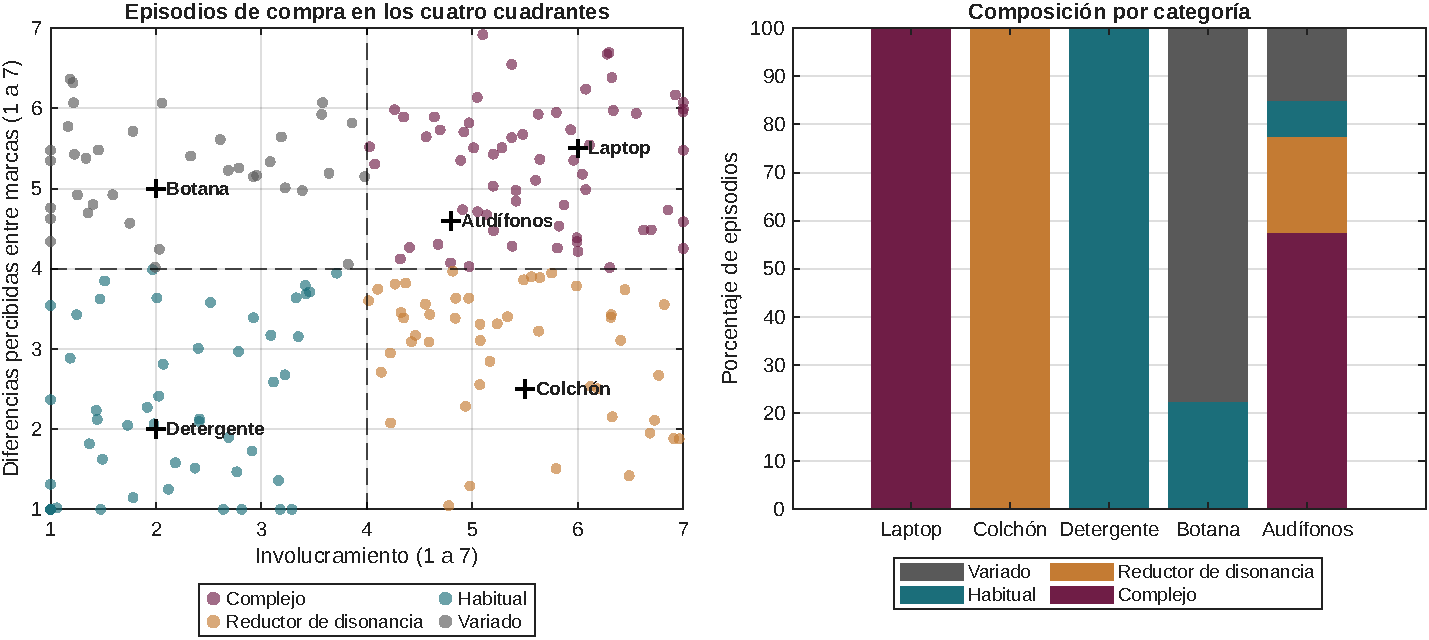
\includegraphics[width=0.98\textwidth]{figuras/matlab/cap09_cuadrantes.pdf}
  \captionof{figure}{Episodios sintéticos en los cuatro cuadrantes y
  composición por categoría. Fuente: elaboración propia con datos sintéticos,
  \texttt{rng(42)}.}
  \label{fig:cap09-cuadrantes}
\end{center}

\begin{center}
  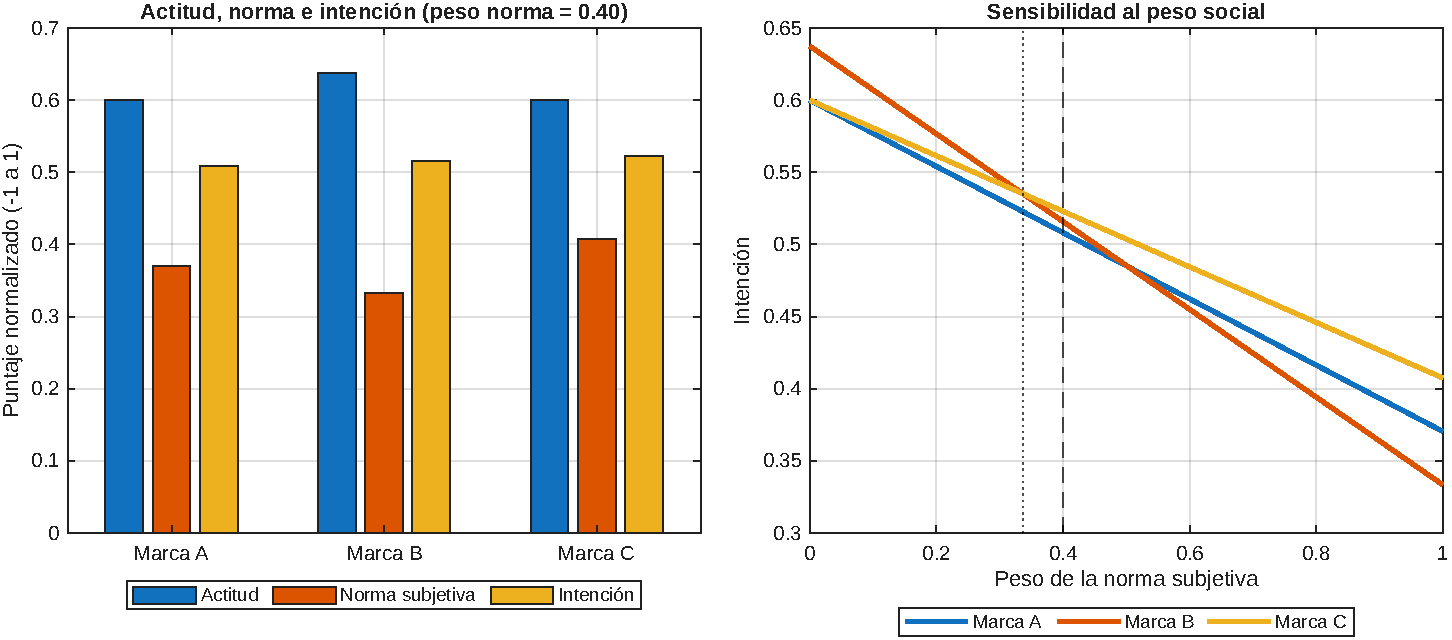
\includegraphics[width=0.98\textwidth]{figuras/matlab/cap09_fishbein.pdf}
  \captionof{figure}{Actitud, norma e intención de tres marcas ficticias, y
  sensibilidad al peso de la norma. Fuente: elaboración propia con datos
  sintéticos.}
  \label{fig:cap09-fishbein}
\end{center}

\textbf{Interpretación de negocio.} Tres lecciones. Primera: el producto no
determina el tipo. Los audífonos, que están cerca de los umbrales, se reparten
entre cuatro tipos, y una campaña pensada para \enquote{el comprador de
audífonos} le habla a una persona que no existe. Segunda: los umbrales son una
decisión del analista, y la distribución cambia cuando se mueven. Tercera: la
marca con mejor actitud no es necesariamente la que gana cuando pesa la
opinión social, y las diferencias de intención pueden ser de unas milésimas,
así que ningún ganador debe presentarse sin su análisis de sensibilidad.

\textbf{Ejercicio propuesto (usen exactamente este script, solo cambien el
bloque de parámetros).} Corran el script tres veces y completen un cuadro con el
porcentaje de cada tipo en la categoría \enquote{Audífonos}, la marca con
mayor intención y el peso de la norma en que cambia la elección:
\begin{enumerate}
  \item \textbf{Caso A — valores por defecto.}
  \item \textbf{Caso B — umbrales exigentes:} \texttt{umbralInvolucramiento = 5},
  \texttt{umbralDiferencias = 5} y \texttt{pesoNorma = 0.10}.
  \item \textbf{Caso C — lo social manda:} \texttt{umbralInvolucramiento = 3},
  \texttt{umbralDiferencias = 3}, \texttt{pesoActitud = 0.20} y
  \texttt{pesoNorma = 0.80}.
\end{enumerate}
Respondan por escrito: ¿qué le pasa a la composición de la categoría
\enquote{Audífonos} al subir o bajar los umbrales, y qué implica para una campaña?
¿Qué marca gana en cada caso y por qué? A partir de las tres corridas, expliquen
por qué una tipología y un modelo de actitud son \emph{ayudas para pensar}, no
mediciones de la realidad.

\textbf{Extensión opcional.} Cambien una \texttt{evaluaciones} (por ejemplo, que
el precio deje de importar con valor 0) y describan cuál es la nueva marca ganadora.
\end{cajaLaboratorio}

\begin{cajaEtica}
Entender cómo decide una persona da poder, y el poder se puede usar bien o mal.
Cuatro cuidados concretos. \textbf{Primero}, no explotar la compra habitual: las
renovaciones automáticas, las casillas premarcadas y los cobros recurrentes
difíciles de cancelar aprovechan que la persona no está evaluando; el
consentimiento y la facilidad de salida son obligaciones, y la LFPDPPP vigente
exige base legal para el tratamiento de datos \parencite{dof_lfpdppp2025}.
\textbf{Segundo}, no inferir motivos sensibles sin necesidad: deducir de los datos que
alguien está en un nivel de necesidad (seguridad, pertenencia) puede llevar a
dirigir ofertas a personas en situación vulnerable, como crédito caro a quien
está en apuros. \textbf{Tercero}, no usar la psicología de la asociación (Pavlov)
para fabricar urgencia falsa. \textbf{Cuarto}, la netnografía exige criterio:
que una publicación sea pública no significa que la persona haya consentido ser
analizada; hay que proteger su identidad, y con más razón si se trata de
personas menores de edad. Un perfil que \enquote{acierta} sobre una
persona también puede estar exponiendo algo que ella no eligió mostrar.
\end{cajaEtica}

\section{Estudio de caso}
\label{sec:cap09-caso}

\begin{casoFicticio}
\textit{Tienda Brisa} es una tienda en línea ficticia que vende audífonos,
detergente, botanas y colchones. Envía a todas sus personas clientes el mismo
flujo de correos: (1) una oferta del 10\,\% por \enquote{terminar tu compra}; (2)
un cuestionario de satisfacción; (3) \enquote{Productos que te pueden gustar}.

Los resultados de un trimestre son éstos: la oferta funciona bien con los
audífonos, mal con el detergente (la gente no lo había dejado en el carrito: lo
compra cada mes), y los colchones tienen la mayor tasa de devolución. Las botanas
se venden en olas: lo que gana un mes pierde el siguiente. El equipo de datos
propone \enquote{un modelo de actitud para todo}.

\textbf{Preguntas guía.}
\begin{enumerate}
  \item Clasifique cada categoría (audífonos, detergente, botanas, colchones)
  en uno de los cuatro tipos y justifique con las firmas de datos del
  cuadro~\ref{tab:cap09-tipos}.
  \item Para cada una, rediseñe el flujo de correos. ¿Qué cambia entre el del
  colchón y el del detergente?
  \item ¿Por qué la oferta de \enquote{terminar tu compra} no funciona con el
  detergente? Use el modelo de Marshall y la tipología.
  \item Comente la propuesta del equipo: ¿en qué categoría tendría sentido un
  modelo de actitud (Fishbein y Ajzen) y en cuál no?
  \item ¿Qué riesgo ético tiene un flujo de recompra automática sin
  recordatorio para el detergente?
\end{enumerate}
\end{casoFicticio}

\section{Actividades y evidencias del portafolio}

El programa pide, para esta unidad, organizadores gráficos con apoyo de
tecnologías de la información, una matriz integradora de los modelos, socialización
en plenaria, solución de casos y prácticas.

\begin{description}
  \item[Organizadores gráficos] Uno por tipo de comportamiento (cuatro) y uno por
  modelo (nueve): una lámina con idea, variable clave, ejemplo digital propio y
  límite. Pueden hacerse con un lienzo digital colaborativo.
  \item[Matriz integradora] Completar las matrices~\ref{tab:cap09-matriz1} y
  \ref{tab:cap09-matriz2} con un \emph{ejemplo propio del equipo} en la
  columna de analítica, con la fuente de cada dato.
  \item[Socialización en plenaria] Cada equipo expone un modelo con el
  caso de Camila, sin repetir el del libro.
  \item[Solución de casos] Resolver por escrito el estudio de caso de
  \textit{Tienda Brisa}.
  \item[Reporte de práctica] Informe de la práctica \enquote{Análisis del
  comportamiento del consumidor} con el cuadro de los casos A, B y C del
  laboratorio y la conclusión propia (la guía formal de las prácticas oficiales de la
  Unidad III se redacta al cerrar la Parte).
\end{description}

\section{Ruta de aprendizaje autónomo}

Cinco horas de aprendizaje autónomo. Tareas concretas:
\begin{enumerate}
  \item \textbf{Clasificar cinco compras propias.} Describir cinco compras
  digitales de los últimos tres meses, clasificar cada una en uno de los cuatro
  tipos y anotar qué indicio (tiempo, búsquedas, regreso al sitio) las sostiene.
  \item \textbf{Un mismo producto, dos episodios.} Encontrar un producto que una
  persona haya comprado una vez como compra compleja y otra como habitual, y
  explicar qué cambió.
  \item \textbf{Un modelo con su corrección.} Elegir uno de los modelos con
  corrección conceptual (Freud/Dichter o Maslow) y escribir media cuartilla
  que distinga lo que el autor dijo de lo que los manuales le atribuyen.
  \item \textbf{Fishbein y Ajzen con datos propios.} Con cuatro atributos y tres
  marcas reales de un producto que usen, estimar creencias y evaluaciones y
  calcular la actitud a mano; comparar con la marca que realmente compran.
  \item \textbf{Netnografía de media hora.} Leer una conversación pública de una
  comunidad sobre un producto, anotar tres temas que no se verían en una
  encuesta y escribir un párrafo sobre qué precauciones éticas tomó.
\end{enumerate}

\section{Síntesis}

El comportamiento de compra se describe con dos ejes (involucramiento y
diferencias percibidas) y cuatro tipos: complejo, reductor de disonancia,
habitual y variado. El tipo pertenece al \emph{episodio}, no al producto, y el
entorno digital puede moverlo. Cada tipo deja una firma distinta en los datos y
pide una táctica distinta. Para explicar \emph{por qué} se compra existen nueve
modelos de orígenes diversos: Marshall (utilidad), Pavlov (asociación), Veblen
(estatus), Freud a través de Dichter (motivos inconscientes), Fishbein y Ajzen
(actitud y norma), O'Shaughnessy (razones y deseos), Maslow (necesidades),
Howard y Sheth (sistema) y la netnografía (método para comunidades en línea).
Dos de ellos exigen corrección sobre lo que los manuales dicen (Freud y Maslow),
uno es método y no teoría, y todos son extrapolaciones cuando se aplican a lo
digital. La pregunta de mercadotecnia decide el modelo; combinar al menos dos y
declarar sus límites es la práctica honesta.

\subsection*{Glosario del capítulo}
\begin{description}
  \item[Actitud multiatributo] Suma de creencia por evaluación sobre los atributos de una marca.
  \item[Consumo conspicuo] Gasto visible cuyo propósito es mostrar estatus (Veblen).
  \item[Disonancia posterior a la compra] Incomodidad de haber elegido entre opciones poco distintas.
  \item[Diferencias percibidas] Cuánto distingue la persona las marcas entre sí, desde su mirada.
  \item[Elasticidad precio] Cambio porcentual de la cantidad demandada entre el cambio porcentual del precio.
  \item[Extinción] Pérdida de una respuesta condicionada cuando el estímulo condicionado deja de acompañarse del incondicionado.
  \item[Intención] Disposición declarada a realizar una conducta; en Fishbein y Ajzen, combinación ponderada de actitud y norma.
  \item[Involucramiento] Importancia que la persona da a una compra, medida por el esfuerzo que invierte en decidir.
  \item[Netnografía] Método cualitativo para estudiar comunidades y culturas de consumo en línea.
  \item[Norma subjetiva] Presión social percibida: suma de creencia normativa por motivación para complacer.
  \item[Umbral de clasificación] Parámetros del script (\texttt{umbralInvolucramiento}, \texttt{umbralDiferencias}): puntaje de 1 a 7 desde el cual se considera ALTO el involucramiento o las diferencias. Rango: real entre 2 y 6; los casos didácticos usan 3, 4 y 5.
  \item[Peso de la norma] Parámetro del script (\texttt{pesoNorma}): peso de la norma subjetiva en la intención. Rango: real entre 0 y 1; se reescala junto con \texttt{pesoActitud} para sumar 1.
  \item[Utilidad marginal] Satisfacción que aporta la última unidad consumida.
\end{description}

\subsection*{Autoevaluación}

\textbf{Opción múltiple}

\begin{enumerate}
  \item Una persona compra un sofá caro; todas las marcas le parecen similares y esa
  noche busca opiniones de la marca que eligió. Es un comportamiento:
  \begin{enumerate}
    \item[a)] Complejo.
    \item[b)] Reductor de disonancia. \textit{(correcta)}
    \item[c)] Habitual.
    \item[d)] Variado.
  \end{enumerate}
  \textit{Justificación:} alto involucramiento y diferencias pequeñas;
  sección~\ref{sec:cap09-disonancia}.

  \item Quien cambia de marca de botana en cada compra, sin queja alguna,
  muestra un comportamiento:
  \begin{enumerate}
    \item[a)] Variado. \textit{(correcta)}
    \item[b)] Habitual.
    \item[c)] Complejo.
    \item[d)] Reductor de disonancia.
  \end{enumerate}
  \textit{Justificación:} bajo involucramiento, diferencias grandes;
  sección~\ref{sec:cap09-variado}.

  \item El tipo de comportamiento de compra es, sobre todo, una propiedad de:
  \begin{enumerate}
    \item[a)] El producto.
    \item[b)] El episodio de compra. \textit{(correcta)}
    \item[c)] La marca.
    \item[d)] El canal.
  \end{enumerate}
  \textit{Justificación:} aclaración 1, sección sobre los dos ejes.

  \item Si el precio sube 20\,\% y la cantidad baja 10\,\%, la demanda es:
  \begin{enumerate}
    \item[a)] Elástica.
    \item[b)] Inelástica. \textit{(correcta)}
    \item[c)] Perfectamente elástica.
    \item[d)] Imposible de calcular.
  \end{enumerate}
  \textit{Justificación:} $\varepsilon=-10/20=-0.5$, $|\varepsilon|<1$;
  sección~\ref{sec:cap09-marshall}.

  \item La pirámide de Maslow, tal como aparece en los manuales:
  \begin{enumerate}
    \item[a)] Está dibujada en el artículo de 1943.
    \item[b)] Es una representación posterior que no aparece en el artículo original. \textit{(correcta)}
    \item[c)] Fue autorizada por Maslow.
    \item[d)] Prueba que las necesidades se satisfacen una por una.
  \end{enumerate}
  \textit{Justificación:} recuadro de corrección,
  sección~\ref{sec:cap09-maslow}.

  \item En la actitud multiatributo, $A=\sum b_i e_i$, la creencia $b_i$ es:
  \begin{enumerate}
    \item[a)] Qué tan bueno es el atributo.
    \item[b)] Qué tan probable es que la marca tenga el atributo. \textit{(correcta)}
    \item[c)] La presión de los amigos.
    \item[d)] El precio.
  \end{enumerate}
  \textit{Justificación:} definición,
  sección~\ref{sec:cap09-fishbein}.

  \item La netnografía es, en rigor:
  \begin{enumerate}
    \item[a)] Un modelo teórico de utilidad.
    \item[b)] Un método de investigación cualitativa. \textit{(correcta)}
    \item[c)] Una prueba A/B.
    \item[d)] Un modelo de condicionamiento.
  \end{enumerate}
  \textit{Justificación:} recuadro,
  sección~\ref{sec:cap09-netno}.
\end{enumerate}

\textbf{Preguntas abiertas}

\begin{enumerate}
  \item Explique por qué Freud no es, en sentido estricto, el autor del modelo
  psicoanalítico de consumo. \textit{Clave:} Freud no escribió sobre consumo;
  Dichter trasladó el psicoanálisis a la investigación motivacional en los
  años cincuenta; la historiografía es cautelosa con su primacía.
  \item Con la figura~\ref{fig:cap09-fishbein}, explique por qué conviene
  reportar el peso en que cambia la elección y no solo un ganador. \textit{Clave:}
  los márgenes son pequeños y los pesos son subjetivos; el análisis de
  sensibilidad lo hace visible.
  \item Dé un ejemplo propio de una interfaz que mueva una compra de un tipo a
  otro y valore si es legítimo. \textit{Clave:} p. ej., el pago de un toque
  pasa de compleja a habitual; legítimo si hay información y opción de
  deshacer, cuestionable si busca anular la deliberación.
\end{enumerate}

\section{Lecturas recomendadas}

\begin{description}
  \item[\textcite{assael1987}] Origen de la tipología de cuatro comportamientos; el libro es de acceso difícil, y es una limitación de este capítulo haberlo contrastado solo con fuentes secundarias.
  \item[\textcite{maslow1943}] El artículo original, corto y legible. Léanlo antes de dibujar la pirámide.
  \item[\textcite{madden1992}] Comparación empírica entre la acción razonada y la conducta planeada; ejemplo de cómo se contrasta un modelo.
  \item[\textcite{kozinets2002}] Referencia central de la netnografía.
  \item[\textcite{simon1955}] Para entender por qué ningún modelo clásico de elección racional describe bien al consumidor real.
\end{description}
